\beginsong{Du machst Kleinholz}[
    wuw={hussa (Werner Helwig), Wolfgang Held (Nerother Wandervogel)}, 
    jahr={1955}, 
    bo={98}, 
    pfii={98}, 
    pfiii={52}, 
    gruen={73}, 
    kssiv={34}, 
    siru={63},
]

\beginverse
\endverse
\centering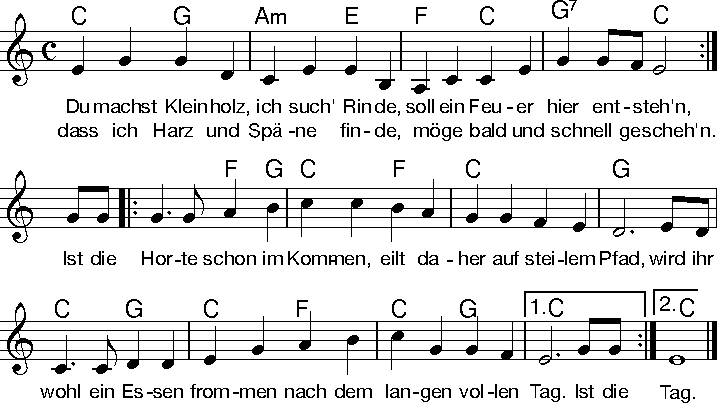
\includegraphics[width=1\textwidth]{Noten/Lied031.pdf}	

\beginverse
\[C]Ich hol' \[G]Wasser, \[Am]du suchst \[E]Schwämme, \[F]leuchten \[C]gelb und \[G]riechen \[C]kalt.
Dass uns \[G]nicht die \[Am]Faulheit \[E]hemme, \[F]geht ein \[C]Regen \[G]durch den \[C]Wald.
\endverse

\beginchorus
Ist die Horte \[G]schon im \[Am]Kommen, \[F]eilt da\[C]her auf steilem \[G]Pfad,
Wird ihr \[C]wohl ein \[G]Essen \[C]frommen, \[F]nach dem \[C]langen, \[G]vollen \[C]Tag.
\endchorus

\beginverse
^Sind das ^Stimmen, ^hörst du ^Rufen? ^Halt die ^Ohren ^in den ^Wind!
Raunt ein ^Bach um ^Felsen^stufen, ^ob das ^wohl die ^Uns'ren ^sind?
\endverse

\renewcommand{\everychorus}{\textnote{\bf Refrain (wdh.)}}
\beginchorus
\endchorus

\endsong
